\documentclass[sigconf,anonymous,balance=false]{aamas}
% AAMAS v2.19 omits its default editors argument and consumes a closing \fi.
% Repair only that exact sentinel with one pending class-loader conditional.
\makeatletter
\def\CIP@missingeditors{\fi}
\let\CIP@classrepair\@empty
\edef\CIP@classloadlevel{\the\currentiflevel}
\ifx\acmConference@editors\CIP@missingeditors
  \ifnum\CIP@classloadlevel=1\relax
    \let\CIP@classrepair\CIP@missingeditors
    \gdef\acmConference@editors{}
  \fi
\fi
\CIP@classrepair
\makeatother
\usepackage{balance}
\usepackage{colortbl}
% Compact table cells use class-defined sizes; body geometry stays official.
\AtBeginEnvironment{table}{\renewcommand{\arraystretch}{0.94}}
\AtBeginEnvironment{table*}{\renewcommand{\arraystretch}{0.94}}
\AtBeginEnvironment{tabular}{\small}
% Unmodified official AAMAS 2027 copyright block and class.
\makeatletter
\gdef\@copyrightpermission{
  \begin{minipage}{0.2\columnwidth}
   \href{https://creativecommons.org/licenses/by/4.0/}{
\includegraphics[width=0.90\textwidth]{by}}
  \end{minipage}\hfill
  \begin{minipage}{0.8\columnwidth}
   \href{https://creativecommons.org/licenses/by/4.0/}{This work is licensed under a Creative Commons Attribution International 4.0 License.}
  \end{minipage}
  \vspace{5pt}
}
\makeatother
\setcopyright{ifaamas}
\acmConference[AAMAS 2027]{Proc.\@ of the 26th International Conference
on Autonomous Agents and Multiagent Systems (AAMAS 2027)}{3--7 May 2027}{Hanoi, Vietnam}{M.~Baldoni, F.~Fang, W.~Yeoh, N.~Yorke-Smith (eds.)}
\copyrightyear{2027}
\acmYear{2027}
\acmDOI{}
\acmISBN{}
\acmSubmissionID{1997}
\submissionType{Research Paper Track}
\title{LLM-Guided Synthesis of Constraint-Adaptive Heuristics for Satellite--Ground Scheduling}
\begin{abstract}
Graph optimization heuristics can achieve strong aggregate performance while relying on decision rules that fail under changes in resource constraints. Effective adaptation requires identifying not only when action preferences should change, but also whether the input representation contains the information needed for that change. We propose an LLM-guided synthesis framework for con\-straint-\allowbreak{}adaptive satellite--ground scheduling that uses certified decision evidence to jointly refine graph representations and ranking rules. Its central mechanism detects ranking requirements that become contradictory under the current feature representation and directs synthesis toward the missing structural distinctions, rather than repeatedly adjusting an insufficient scoring interface. Two complementary mechanisms support this refinement. First, controlled offline interventions on resource-constraint configurations generate paired static scheduling problems in which the same competing actions remain individually feasible. Sound bounds on conditional completion values certify preference reversals or preservation under explicit boundary commitments, yielding relational specifications of when rankings should change or remain stable. Second, structural witnesses guide the LLM to compose distinguishing features from a typed graph-operation library and synthesize corresponding ranking rules. Feature--rule pairs are selected jointly for finite input representability, preference fit, complete-schedule quality, and feature-computation cost, making representation expansion targeted and cost-aware. We formulate contact selection as maximum-weight independent set optimization and study adaptation using a frozen program on held-out scheduling instances and constraint configurations. The synthesized program responds to the current conflict graph within a fixed feasibility-enforcing kernel, without online LLM or full-residual certification-oracle calls. By linking representation refinement to certified decision conflicts, the framework addresses information limitations beyond rule-only repair while explicitly accounting for the computational cost of constraint adaptation.

\end{abstract}
\keywords{Satellite scheduling, maximum-weight independent set, heuristic synthesis, representation refinement, large language models}
\ccsdesc[500]{Computing methodologies~Planning and scheduling}
\ccsdesc[300]{Mathematics of computing~Combinatorial optimization}
\begin{document}
\maketitle
% V06 integrates completed, independently audited frozen-result analyses.
\begin{figure*}[t]
\centering
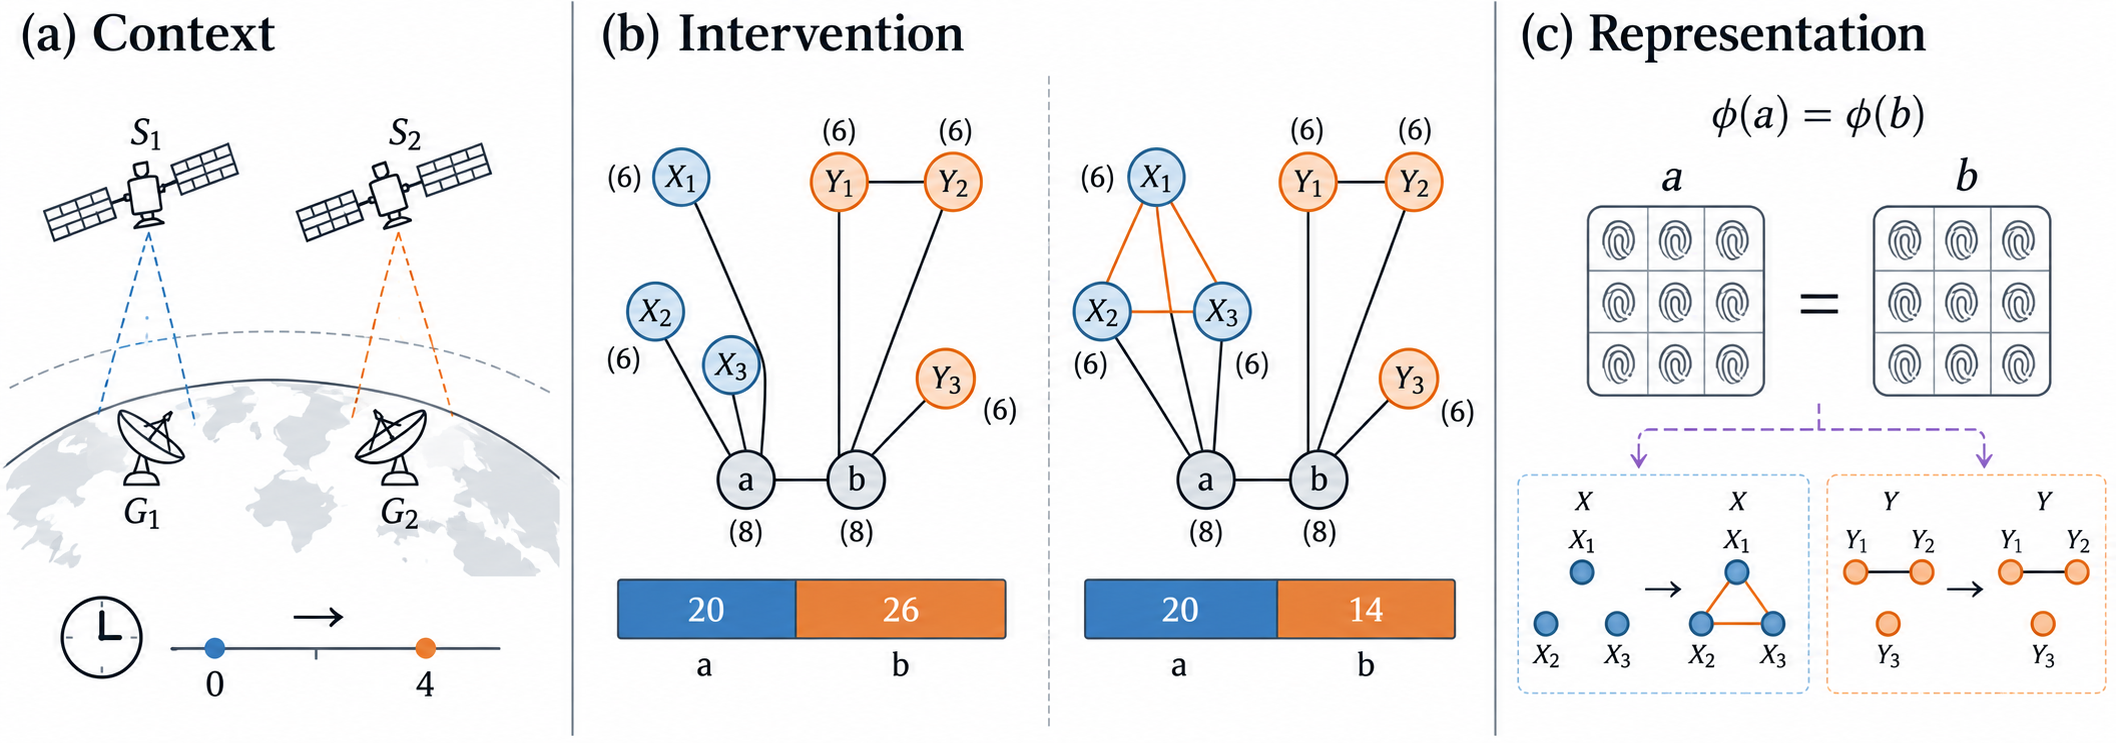
\includegraphics[width=.70\textwidth]{figures/context_evidence_v05.png}
\Description{A constructed aligned contact pair changes compatibility under a ground-gap intervention. Two base-feature-equivalent competing actions remain individually feasible, while their full conditional-completion preferences reverse.}
\caption{\textbf{Constraint adaptation can require new information.} Forced-completion increments of $a,b$ change from $20,26$ to $20,14$ in this constructed example, reversing preference despite equal nine-input vectors within each configuration. The common fixed reward is excluded; structural compatibility supplies the missing distinction.}
\label{fig:motivation}
\end{figure*}
% Root review of independently authored V06 section; original preserved.
\section{Introduction}
\label{sec:introduction}
A satellite--ground contact excludes opportunities sharing its resources.
Changing a switching gap changes which alternatives can coexist, and hence
their opportunity costs, while preserving contacts and rewards.
We isolate the static pairwise-conflict subproblem as maximum-weight
independent set (MWIS)~\cite{augenstein2016optimal,levinson2025optimal}
and study a reusable heuristic across resource configurations.

LLM synthesis searches executable heuristics through evaluation and
reflection~\cite{romeraparedes2024funsearch,liu2024eoh,ye2024reevo}.
Aggregate reward does not identify whether failure needs a different formula
or missing input information. No pointwise rule can satisfy incompatible
strict preferences over identical observations.

Figure~\ref{fig:motivation} illustrates this obstruction. Two competing contacts
have identical nine-input vectors within each configuration. Their
forced-completion increments change from $20,26$ to $20,14$ after a ground-gap
intervention, reversing preference while both contacts remain individually
feasible. A base-only scalar necessarily ties them; neighborhood compatibility
supplies the missing distinction. These illustrated values exclude the common
fixed reward and are conditional optima, not heuristic rollout returns.

We propose \emph{certified representation--rule refinement}. Offline interventions
preserve contacts and explicit boundary commitments. Sound bounds certify
full-residual preference reversals or preservation; unresolved comparisons abstain.
Identical residual components cancel within each configuration. The resulting
strict requirements are projected onto exact feature-equivalence classes.
A directed cycle proves that every scalar on the interface is insufficient.
Its concrete ranking arcs and equality joins identify occurrences that must be
distinguished, adapting abstraction-refinement
principles~\cite{clarke2000cegar,frances2021policies} to optimization decisions.

We use an LLM as a conditionable proposal operator in the combinatorial space
of bounded typed graph computations and score expressions. Witnesses identify
necessary distinctions without supplying their computation, conditioning
generation on an information deficit. Deterministic search remains viable:
our supplied 53-expression TRAIN catalogue admits exact minimum-additive-cost
repair. The theory motivates refinement; proposer efficiency remains empirical.

Splitting one witness can expose another, requiring complete-quotient rechecks.
TRAIN selection checks acyclicity, scalar fit, scheduling quality and work
before freezing. Priorities control greedy additions and pivots in shared
classical repair~\cite{lamm2019weighted,grossmann2025chils}; repeated deployment
needs no LLM or full-residual certification calls.

Our contributions are:
\begin{enumerate}
\item \textbf{Information diagnosis:} finite pointwise representability with
concrete cycle witnesses, separating insufficient inputs from poor rule fit.
\item \textbf{Targeted cost-aware synthesis:} certified completion requirements
and equality joins direct typed feature--rule refinement, with full-quotient
rechecks and a finite-catalogue additive-cost guarantee.
\item \textbf{Frozen evaluation:} evidence-controlled authoring, separate
representability and scalar-fit measurements under a common kernel,
and separate published-solver comparisons.
\end{enumerate}
Shared-seed TRAIN repair yields 26/32 information-compatible W proposals
versus 19/32 with relations alone. Joint selection raises withheld fit within
W by 3.37 points, while relations-only outputs retain stronger fit.
Scheduling improvement remains separate and is tested against published solvers.

% Root review of independently authored V06 section; original preserved.
\section{Related Work}
\label{sec:related}
Satellite scheduling couples observation, downlink and shared ground
resources~\cite{augenstein2016optimal,levinson2025optimal,picard2021constellations}.
Graph learning guides constructive optimization and exact
search~\cite{khalil2017learning,li2018gcn,gasse2019exact}; local topology can aid
neural generalization~\cite{bai2025local}. Our question concerns whether an
interface can express certified decision requirements before fitting a scorer.

\paragraph{LLM design.}
FunSearch combines generated programmes with executable evaluation;
EoH evolves descriptions and code; ReEvo and LLaMEA add reflective or evolutionary
fitness feedback~\cite{romeraparedes2024funsearch,liu2024eoh,ye2024reevo,vanstein2025llamea}.
A$_2$DEPT evolves complete solvers with hierarchical edits,
while PathWise carries derivation history through a search-memory
graph~\cite{chen2026a2dept,gungordu2026pathwise}. Their open-ended programmes can
introduce structural computations, so feature invention alone is not our
contribution. We supply certified contradictions in the current interface and
concrete equality joins to direct that invention. DRAGON uses decomposition and
reconstruction agents during optimization~\cite{chen2026dragon}; here an offline
LLM yields a frozen priority inside classical search. Dynamic heuristic selection
and algorithm configuration optimize state-dependent choices and
settings~\cite{speck2021dynamic,hutter2009paramils}; we refine the available
input distinctions and account for their computation.

\paragraph{Representation and synthesis.}
GNN expressiveness connects architectural distinctions to graph isomorphism
tests~\cite{xu2019powerful,morris2019weisfeiler}. Our quotient instead collapses
exactly equal observed feature vectors. Generalized planning learns features,
representations and policies shared across
instances~\cite{bonet2018representation,bonet2019features,frances2021policies}.
CEGAR and abstraction-guided synthesis refine abstractions after
counterexamples~\cite{clarke2000cegar,wang2018abstraction}; sketching,
syntax-guided and relational synthesis separate syntax from semantic
obligations~\cite{solarlezama2006sketch,alur2013sygus,wang2018relational}.
Our requirements are sound conditional preferences made contradictory by
information collapse, rather than spurious abstract executions. Equality joins
identify distinctions needed before rule fitting. Finite representability,
bounded-grammar fit and deployment effectiveness remain different properties.

\paragraph{Classical MWIS and evaluation.}
Independent-set exchanges and clique-based branch-and-bound provide
foundations~\cite{andrade2012local,ostergard2002clique}. Published weighted solvers
include concurrent CHILS search, multilevel M$^2$WIS, Struction transformations
and WeightedBR~\cite{grossmann2025chils,grossmann2024mmwis,gellner2021struction,lamm2019weighted}.
These mature components support our common kernel and separate algorithm
comparisons; they are not claimed as new search primitives. Artificial weights
can favor particular heuristics and inference rules~\cite{mccreesh2017evaluation}.
We therefore include application-derived public weighted graphs, preserving
objectives through exact transformations and reporting numerical compatibility.

% Root review of independently authored V06 section; original preserved.
\section{Problem Setting}
\label{sec:problem}
A contact $v$ specifies satellite $\sigma_v$, station $\gamma_v$, interval
$[s_v,e_v)$, with $s_v<e_v$, and nonnegative reward $w_v$. Selection reserves that entire
interval. Each main-model satellite and station has capacity one. For contacts
ordered by start, a shared station conflicts if $s_v<e_u+\tau_g$; a shared
satellite uses $s_v<e_u+\tau_s$. Nonnegative switching gaps are fixed within
configuration $\theta$. Synthetic reward is independent of duration.
The weighted conflict graph $G_\theta=(V,E_\theta,w)$ yields
\begin{equation}
 \max_{\substack{I\subseteq V\\ I\text{ independent in }G_\theta}} w(I),
 \qquad w(I)=\sum_{v\in I}w_v.
 \label{eq:mwis}
\end{equation}
This models constraints expressible by pairwise conflicts. Public graphs
exercise MWIS without a satellite interpretation; exploratory C3 tracks retain
their separate inherited predicates.

An admissible boundary $B=(F,X)$ records independent permanent commitments
$F$, disjoint from permanent exclusions $X$. Available contacts are
\begin{equation}
 R_\theta(B)=V\setminus(F\cup X\cup N_\theta(F)).
 \label{eq:residual}
\end{equation}
For $d\in R_\theta(B)$, its full conditional-completion value is
\begin{equation}
 V_\theta(d\mid B)=
 \max_{\substack{I\subseteq V\text{ independent in }G_\theta\\
                 F\cup\{d\}\subseteq I,\ I\cap X=\varnothing}}w(I).
 \label{eq:conditional-value}
\end{equation}
It includes fixed reward and every compatible global completion.
An aligned intervention changes one constraint parameter while preserving
contacts, resources, intervals, weights and boundary. The common boundary must
be admissible under both configurations. Competing $a,b$ must
remain available and adjacent in both configurations. Their certified
preferences can change even though each remains individually feasible.
Adaptation compares separate static problems, not online constraint changes.

A frozen deterministic typed programme $P=(\phi_P,h_P)$ gives finite priorities
$h_P(\phi_P(G_\theta,A,v))$ on active snapshot $A$.
All programmes share an initializer, patch rules, classical search and
feasibility checks. They alter greedy additions and pivots, which can change
later repair trajectories. The kernel protects $F$, avoids $X$, retracts only
movable incumbent vertices and commits only globally feasible positive gains.
Budget termination retains a feasible incumbent, not necessarily an optimum.
Full-residual labels and restricted-patch search have different temporary
commitments; ranking agreement and schedule quality require separate evaluation.

\begin{figure*}[t]
\centering
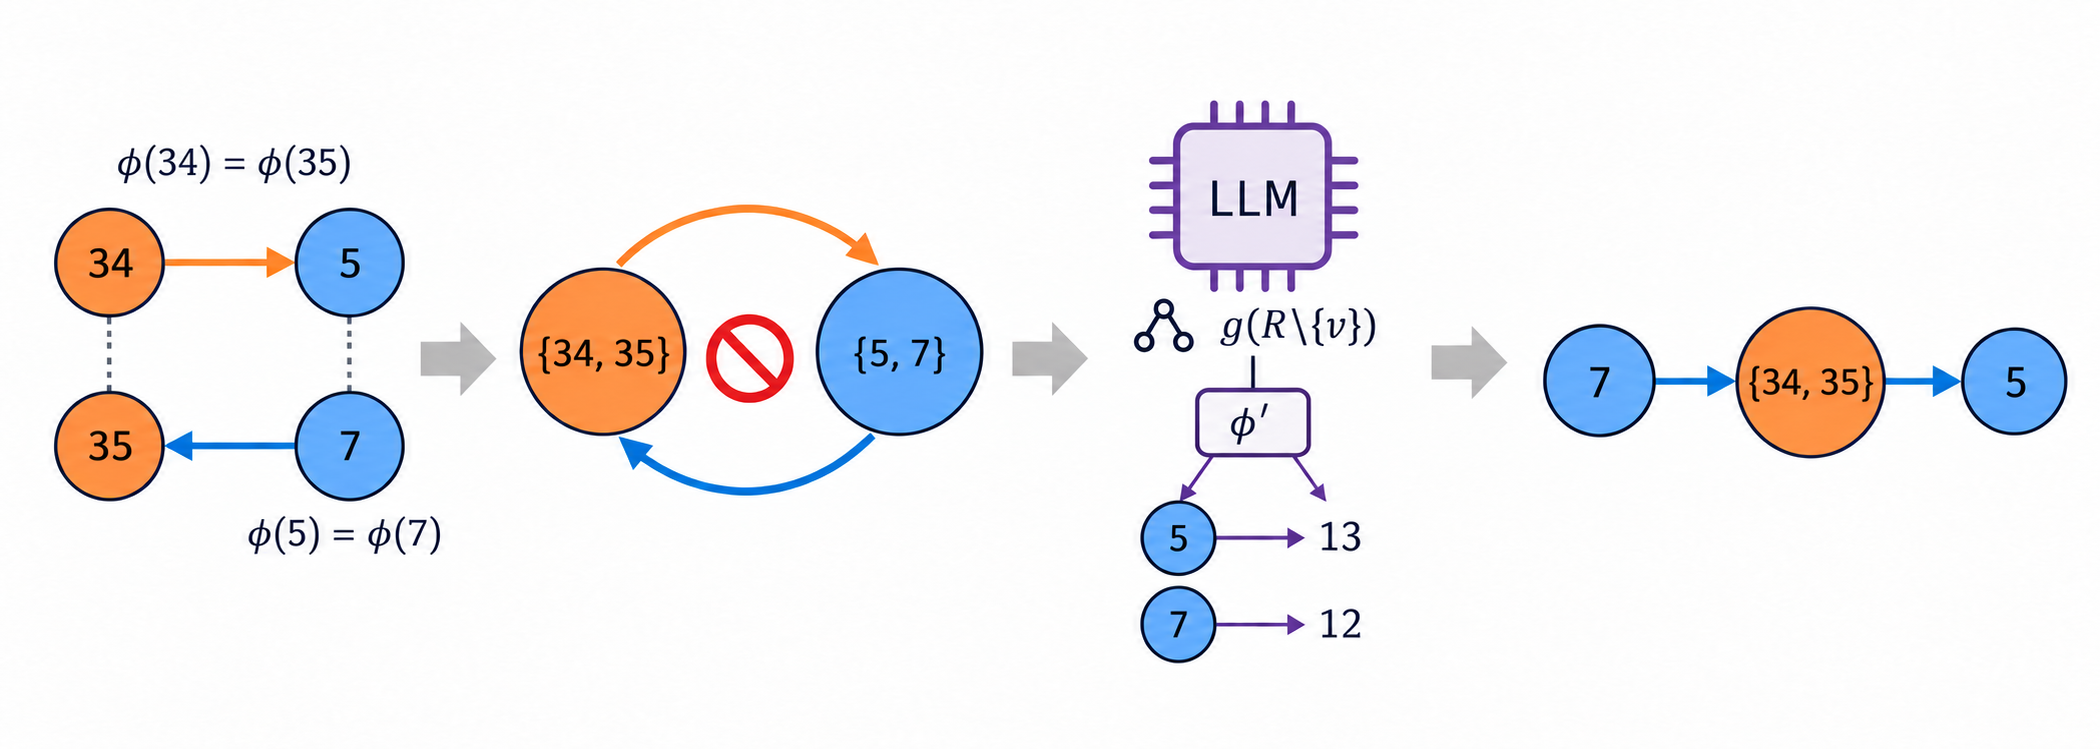
\includegraphics[width=.72\textwidth]{figures/quotient_cycle_replacement_v06.png}
\Description{Two certified strict arcs become a directed two-cycle through equality joins of a rejected interface. Replacing a feature with a typed root-deletion packing computation distinguishes the responsible occurrences, removing this displayed obstruction.}
\caption{\textbf{A structural witness tells synthesis what to distinguish.} In a real TRAIN seed, requirements $34\!>\!5$, $7\!>\!35$ and joins $5\sim7$, $34\sim35$ create a two-cycle. Replacing a coordinate with the recorded cold-bank root-deletion feature separates $5,7$ (feature values $13,12$), removing this obstruction. Joint selection still rechecks the complete inventory.}
\label{fig:method}
\label{fig:repair}
\end{figure*}
\begin{figure*}[t]
\centering
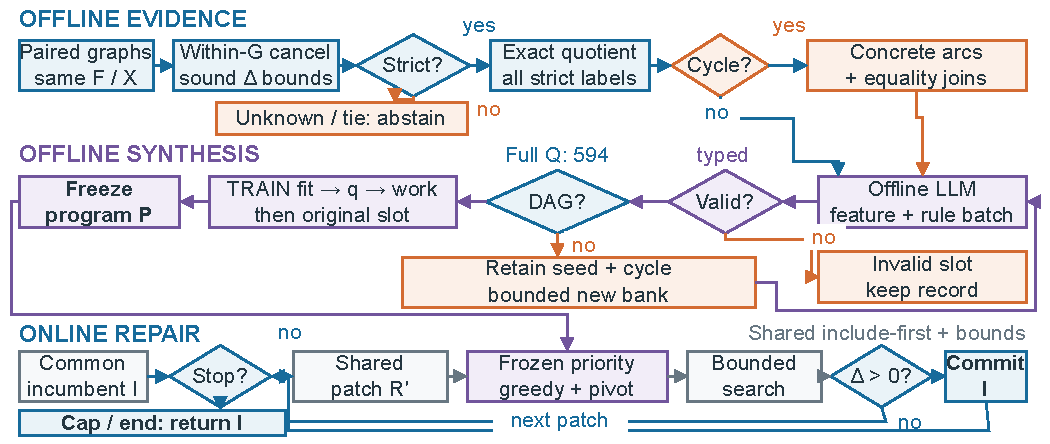
\includegraphics[width=.84\textwidth]{figures/algorithms_v06c.pdf}
\Description{Offline sound certificates feed complete-quotient diagnosis. Concrete equality joins direct typed LLM feature-rule proposals, followed by full quotient, rule-fit, scheduling and cost checks. Frozen priorities operate inside a common feasibility-enforcing repair kernel without online model or certification calls.}
\caption{\textbf{Offline refinement and shared deployment.} Quotient witnesses guide typed proposals; joint selection checks representability, scalar fit, reward and work before freezing. Priorities guide greedy additions and pivots within common feasible classical search. R2 tests one bounded warm-repair round of this general procedure.}
\label{fig:algorithm}
\end{figure*}
% Root review of independently authored V06 method; original preserved.
\section{Certified Representation--Rule Refinement}
\label{sec:method}
Figure~\ref{fig:algorithm} separates certified preferences, quotient-guided
feature--rule synthesis and frozen execution in a common bounded kernel.

\subsection{Full-Residual Decision Evidence}
\label{sec:method:certificates}
At boundary $B=(F,X)$, put $A=R_\theta(B)$ and
$A_d=A\setminus(\{d\}\cup N_\theta(d))$. Let $\mathcal C_d$ be the connected
components of $G_\theta[A_d]$, identified by complete vertex sets. Then
\begin{equation}
 V_\theta(d\mid B)=w(F)+w_d+
             \sum_{C\in\mathcal C_d}\alpha_w(G_\theta[C]),
 \label{eq:component-completion}
\end{equation}
where $\alpha_w$ is the MWIS optimum. Within one graph and boundary, set
$\mathcal A=\mathcal C_a\setminus\mathcal C_b$ and
$\mathcal B=\mathcal C_b\setminus\mathcal C_a$; identical components cancel:
\begin{equation}
 \Delta_{ab}=w_a-w_b+\sum_{C\in\mathcal A}\alpha_w(G_\theta[C])
                        -\sum_{C\in\mathcal B}\alpha_w(G_\theta[C]).
 \label{eq:cancelled-difference}
\end{equation}
Sound component intervals $[L_C,U_C]$ give
\begin{equation}
 \begin{split}
 \underline\Delta_{ab}&=w_a-w_b+\sum_{C\in\mathcal A}L_C-\sum_{C\in\mathcal B}U_C,\\
 \overline\Delta_{ab}&=w_a-w_b+\sum_{C\in\mathcal A}U_C-\sum_{C\in\mathcal B}L_C.
 \end{split}
 \label{eq:difference-envelope}
\end{equation}
\paragraph{Lemma 1 (within-graph cancellation).}
The endpoints enclose the full conditional-completion difference.
\emph{Proof.} Component optima unite feasibly; identical induced components
cancel. Bounds on remaining signed terms give the enclosure.\hfill$\square$

Cancellation requires identical vertex sets within the same graph, not equal
size or weight; overlapping components remain separate. Verified packings
give lower bounds and clique partitions give upper bounds by summing clique
maximum weights. Bounded exact search tightens intervals; unsearched components
retain $[0,w(C)]$. Rational arithmetic and outward display rounding preserve
soundness; unresolved comparisons abstain.

Certify aligned configurations separately. For $\epsilon\geq0$,
$\underline\Delta^{\theta_0}_{ab}>\epsilon$ and
$\overline\Delta^{\theta_1}_{ab}<-\epsilon$ certify reversal; equal strict
signs certify preservation. Ties impose no strict requirement. Certified pairs
require
\begin{equation}
 h(\phi(x^+))>h(\phi(x^-)),\qquad x=(G_\theta,A,v).
 \label{eq:strict-requirement}
\end{equation}
Each label retains its graph, boundary, actions and signed bounds.

\subsection{Complete Quotients and Structural Witnesses}
\label{sec:method:repair}
Merge occurrences with exactly equal represented values under frozen
semantics. Quotient $Q_\phi$ has one vertex per class and an arc
$[x^+]\to[x^-]$ for every strict requirement, including self-loops.
The base nine coordinates are reward, duration, degree, neighbor-weight
sum/maximum, compatible-weight sum, ground/satellite gaps and residual count;
explicit IDs and dataset labels are excluded.

\paragraph{Theorem 1 (finite pointwise representability).}
An unrestricted deterministic scalar $h(\phi(x))$ satisfies all observed
requirements if and only if $Q_\phi$ is acyclic.
\emph{Proof.} A directed cycle demands a strict decrease back to the same
vector. On a finite DAG, each class's longest outgoing-path length strictly
decreases along every arc. Scaling gives any positive margin.\hfill$\square$

Observed-vector existence implies neither bounded-grammar expressibility
nor unseen correctness. A cycle stores concrete
arcs $p_i\to n_i$ and equality joins $n_i\sim_\phi p_{i+1}$, with cyclic
indices (Figure~\ref{fig:repair}); a repair must split a join. Joins can cross
configurations or boundaries, making statewise checks insufficient. Splitting
one witness can expose another; each proposal rebuilds the \emph{complete}
quotient over all retained requirements.

\subsection{Scoped Minimum-Cost Interface Repair}
Fix the base, evidence and occurrence feature table. For finite catalogue
$\mathcal F$, positive standalone costs $c_f$ and limit $K$, set $d_{Wf}=1$
when $f$ splits a join of witness $W$. The optional exact master is
\begin{equation}
 \begin{split}
 \min_{z\in\{0,1\}^{|\mathcal F|}}\quad&\sum_f c_fz_f,\\
 \text{subject to}\quad&\sum_f d_{Wf}z_f\geq1\quad(\text{retained }W),\\
 &\sum_fz_f\leq K.
 \end{split}
 \label{eq:repair-cover}
\end{equation}
Globally solve each master and rebuild the entire quotient from the base and
selected additions. A surviving cycle adds a cut; subsequent solutions can
replace additions. Refined cycles can revisit coarse classes, so splitting
only the original witness is insufficient.

\paragraph{Theorem 2 (finite-catalogue additive optimum).}
An acyclic terminating solution minimizes additive cost among catalogue
repairs satisfying $K$.
\emph{Proof.} Every acyclic repair splits a join of each retained witness,
satisfying all cuts. Exact master cost lower-bounds valid repairs; the final
DAG attains it. Each cut excludes the current cyclic subset. Finitely many
subsets imply termination or infeasibility under unrestricted search.\hfill$\square$

Inseparable witnesses and truncated masters remain unresolved. This guarantee
covers fixed evidence and additive standalone work, not shared-DAG runtime
or scalar fit. Practical proposal banks do not inherit master optimality.

\subsection{Typed Feature--Rule Proposals}
\label{sec:method:features}
\paragraph{Why use an LLM?}
A witness diagnoses joins to split without constructing a distinguishing
computation and compatible score. Typed graph operations, reductions and
score expressions create a combinatorial programme space. The LLM supplies
a witness-conditioned proposal operator~\cite{romeraparedes2024funsearch,liu2024eoh};
deterministic quotient, scalar-fit and execution checks retain authority.
Theorem~1 requires representation refinement, not an LLM. The fixed-catalogue
procedure is a deterministic alternative once expressions are available.

The offline grammar permits active, neighbor, root-deleted and compatible
continuation sets, typed union/intersection/difference, and count, weight-sum,
edge-count, greedy-packing and clique-cover reductions. Arithmetic and
conditionals combine scalars. Static validation enforces types, bounded syntax
and deterministic operations rather than unrestricted executable code.

\paragraph{Constructing a distinguishing programme.}
The request supplies graph snapshots, certified relations, concrete joins,
the current programme and typed grammar. For an illustrative construction,
not a learned winner, let $D_v=A\setminus\{v\}$ and
$C_v=A\setminus(N(v)\cup\{v\})$. Valid packing and induced-edge reductions give
\begin{equation}
 \begin{aligned}
 f_p(v)&=g(C_v),\qquad f_e(v)=|E[D_v]|,\\
 h(v)&=w_v+\alpha f_p(v)-\beta f_e(v)/(1+\deg(v)),
 \end{aligned}
 \label{eq:typed-construction}
\end{equation}
where $g$ is greedy-packing weight and $\alpha,\beta$ are bounded constants.
Continuation packing measures coexistence; root deletion exposes residual
structure. Actual join splitting and score signs still require complete-inventory
checks. The LLM constructs expressions and rules together; the catalogue
master selects existing expressions.

The information gate uses all nine base coordinates and only added features
referenced by the rule; unused additions cannot repair it. All declarations
must pass finite-value checks. Shared expression DAGs and branch-sensitive
evaluation avoid redundant work. Priorities are computed once per immutable
patch snapshot; initialization and feature queries are charged.

\subsection{Shared Classical Execution and Joint Selection}
\label{sec:method:execution}
All conditions share Degree initialization or a charged CHILS
incumbent~\cite{grossmann2025chils}, then a bounded clique-bound repair kernel.
Feasible incumbents, weighted bounds and local improving replacements are
standard MWIS primitives
\cite{lamm2019weighted,gellner2021struction,grossmann2024mmwis}.
These shared components are not our contribution. Imported incumbents must
be independent, include
permanent $F$ and exclude $X$.
For independent incumbent $I$, destroy movable $D\subseteq I\setminus F$ and
retain $F_{\rm out}=I\setminus D$. A patch satisfies
$D\subseteq R'\subseteq V\setminus(F_{\rm out}\cup N(F_{\rm out})\cup X)$.
Branch-and-bound searches independent replacements in $R'$; only checked
positive exact gains are committed. The programme controls greedy additions
and pivots; targets, patches, bounds and include-first traversal remain common.
Caps retain the feasible incumbent.
Full-residual labels do not certify restricted-patch preferences.

\label{sec:method:selection}
Eligibility requires finite validated syntax, an acyclic demanded quotient
and feasible error-free TRAIN execution. Strict fit $m(P)$ counts requirements
whose score difference exceeds $\eta\geq0$. For family state sets $\mathcal D_t$,
use
\begin{equation}
 q(P)=\frac1{|\mathcal T|}\sum_{t\in\mathcal T}\frac1{|\mathcal D_t|}
       \sum_{G\in\mathcal D_t}\frac{w(I_P(G))}{w(V_G)}.
 \label{eq:train-macro-quality}
\end{equation}
This is total-input-reward fraction, not optimum percentage; zero-total states
use one. Feature-plus-repair work $c(P)$ uses the same averaging. Eligible
selection maximizes $m$, then $q$, minimizes $c$, then uses original slot.
Empty banks have no replacement. Quality-only baselines maximize $q$, then
minimize $c$, without a gate. Budgets, ASTs and selectors freeze on TRAIN.
Measured CPU/wall accompany the work proxy; deployment calls neither LLM nor
full-residual certification oracle.

% Completed TRAIN findings; frozen evaluation fragments are included below.
\section{Experiments}
\label{sec:experiments}

We distinguish representability, scalar fit and scheduling performance.
All conditions share the typed library and classical kernel; shared-search
gains alone do not establish LLM-guidance benefit.

\subsection{Decision Evidence and Authoring Design}
TRAIN contains 120 unit-weight states with at most 32 vertices: 24
source-induced public graphs and 96 contact endpoints forming 48 intervention
pairs. Public clusters are partitioned within a previously exposed corpus.
Contact pairs preserve opportunities and change only ground switching gap,
$0\!\to\!1$; satellite gap remains zero and capacities one.
Queries precede certification and retain shortfalls. Of 1,503 comparisons,
594 are strict, 909 tie and none are unknown; 90 strict comparisons alias
under base-nine vectors. Among 630 paired queries, 12 reverse and 123
preserve strict preferences, 294 tie on both sides and 201 have one tied
endpoint. This controlled,
alias-enriched frame diagnoses conflicts, not their natural incidence.

R2 repairs a shared rejected interface and cycle. Prompts show six cases and
eleven relations; checking retains all 594 requirements. Five blocks contain
eight proposals per W/R/O arm; the first four form the preregistered matched
cohort and the fifth remains reported. Authoring requests
\texttt{gpt-6.1-sol}/ultra; the served backend is undisclosed.
All 120 programs complete server TRAIN assessment with feasible incumbents.
Matched slots do not match compute.

\subsection{What Witness Feedback Repairs}
Matched information-gate yield is 26/32 W versus 19/32 R, a 21.875-point
difference (Table~\ref{tab:v06-authoring}). The table also retains the complete
five-block cohort; Figure~\ref{fig:v06-yield} plots all five bank counts per
arm against measured author-call wall cost.
These are conditional interface repair findings, not general model efficacy.

\begin{table}[t]
\centering
\fontsize{9}{10.4}\selectfont
\setlength{\tabcolsep}{3pt}
\caption{R2 information-gate yield: eligible/original positions in all five
blocks and the preregistered matched four. Bold marks observed column bests.}
\label{tab:v06-authoring}
\begin{tabular}{lrr}
\toprule
Arm & All five & Matched four\\
\midrule
\textbf{W} & \textbf{28/40} & \textbf{26/32}\\
R & 24/40 & 19/32\\
O & 0/40 & 0/32\\
\bottomrule
\end{tabular}
\end{table}
\begin{figure}[t]
\centering
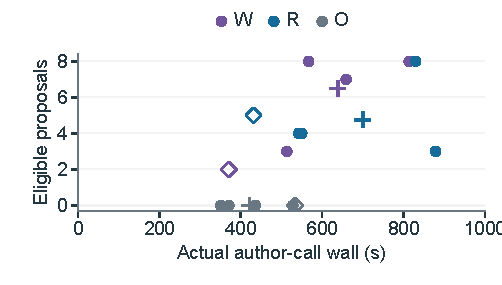
\includegraphics[width=.92\columnwidth]{figures/refinement_authoring_efficiency_v06.pdf}
\Description{Gate-eligible proposals and measured author-call wall time for all five banks in every arm. The fifth bank is distinguished rather than removed.}
\caption{LLM proposal efficiency: eligible proposals versus actual
author-call wall time. All five banks remain shown; the fifth is hollow
and matched means are crosses. Times describe whole calls.}
\label{fig:v06-yield}
\end{figure}

Matched W/R banks produce 10.18/6.78 eligible proposals per 1,000 measured
author-call seconds, descriptively conditional on this seed and these calls.
The gate measures whether the demanded features admit a consistent ordering;
it does not certify the authored scalar or scheduling benefit. Detailed scalar
fit, feature work and policy quality remain in the supporting report and
Discussion, separate from information repair.
All TRAIN schedule qualities equal $2693/4480$ under Eq.~\ref{eq:train-macro-quality};
there is no observed TRAIN reward improvement, before any distribution shift.

Deployment freezes four genuine W joint and twelve matched quality-only
selections before TEST certification; evaluation outcomes select no winner.
Joint-versus-quality contrasts include selection, not isolated witness effects.

\subsection{Complete Quotient Checking and Feature Cost}
The optional catalogue contains all 53 canonical expressions from valid
cold authoring, adaptively discovered on TRAIN, with the same 594 requirements
and $K=6$. Its 4/8/16-expression prefixes remain cyclic. The full catalogue
resolves the quotient using four features at exact minimum additive cost
1,371,468; a verified nonnegative weighting of necessary cuts proves the
matching lower bound.

Seven self-loop cuts precede two cycle cuts: removing self-loops leaves a
cycle, and splitting it exposes another, requiring the ninth full-inventory
check (Figure~\ref{fig:v06-catalogue}). Greedy tie orders remain
identifier-sensitive. This certifies scoped representation repair and an
additive feature-work proxy, not a fitted scalar or runtime optimum.

\begin{figure*}[t]
\centering
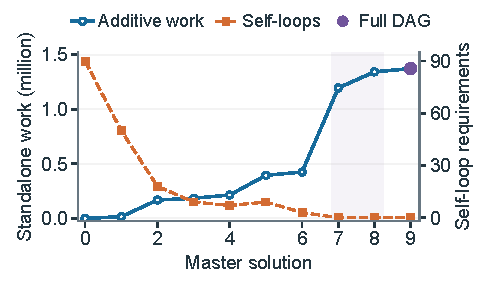
\includegraphics[width=.45\textwidth]{figures/refinement_cost_curve_v06.pdf}\hfill
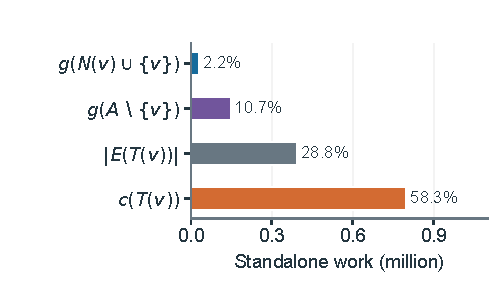
\includegraphics[width=.45\textwidth]{figures/refinement_feature_work_v06.pdf}
\Description{Full-quotient obstructions and additive feature work across catalogue trials; work composition of the certified four-feature minimum.}
\caption{TRAIN catalogue repair: full-quotient obstructions and additive
cost (left), minimum-cost feature work (right). Cyclic trials are not repairs.
Standalone work excludes shared-DAG savings and complete-policy cost.
$g(S)$ is greedy-packing weight, $T(v)=A\setminus(\{v\}\cup N(v))$,
and $c(S)$ is clique-cover upper-bound weight.}
\label{fig:v06-catalogue}
\end{figure*}

\subsection{Published Solvers and Common Components}
Stochastic native solvers use three fixed seeds; deterministic methods and
Degree use one. Exact transformations preserve objectives; signed-range
incompatibilities remain nulls. Coverage and actual costs accompany rewards;
nominal targets are not end-to-end hard deadlines.

EoH-DSL~\cite{liu2024eoh} adapts published operators in four runs of eight
genuine calls with a two-member distinct-quality population. The typed interface
and common rejected seed delimit this reproduction. Its four frozen deployment
identities retain the shared seed; full TRAIN fitness and authoring cost are
reported in the supporting material and Discussion. Authoring compute is not
matched to R2.

\subsection{Adaptation to Withheld Constraint Configurations}
\label{sec:v06-heldout}

\begin{figure*}[!t]
\centering
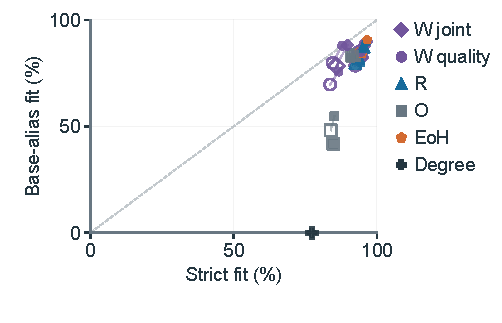
\includegraphics[width=.45\textwidth]{figures/heldout_strict_alias_movement_v06.pdf}\hfill
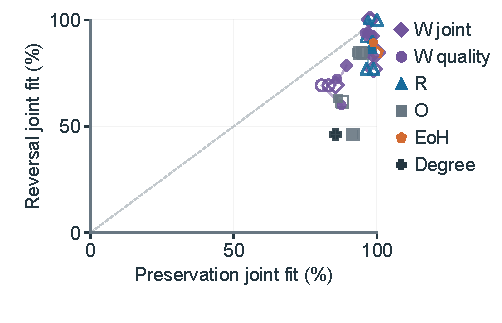
\includegraphics[width=.45\textwidth]{figures/heldout_pair_joint_movement_v06.pdf}
\Description{Strict versus base-alias scalar fit and strict-preservation versus strict-reversal joint correctness for the 21 predeclared main identities. Hollow points are original observations; solid points are the complete five-rename means, with thin connectors retaining movement.}
\caption{Frozen preference transfer: strict versus base-alias fit (left),
strict-preservation versus strict-reversal correctness (right). Hollow/solid
points denote original/five-rename means of all 21 predeclared identities;
coincident identities and renamings remain dependent.}
\label{fig:v06-heldout}
\end{figure*}

The mechanism TEST contains 24 source-disjoint public states and 48 newly
drawn contact endpoints forming 24 pairs. Contact generation retains TRAIN's
resource regimes and unit weights, but uses new seeds and withheld gaps
$0.25\!\to\!2$. Within a pair, the same contacts induce two conflict graphs.
All four W-joint rules omit the available gap coordinates and recompute
structural features from the current graph. No TEST preference label enters
their scoring. Certification occurs after the program
freeze and supplies evaluation targets only.

We evaluate 31 frozen identities and five prescribed identifier renamings.
Of 962 comparisons, 453 are strict (including 79
base-nine aliases) and 509 are exact ties. The 355 paired queries comprise
13 strict reversals, 83 strict preservations, 130 ties on both endpoints and
129 with one tied endpoint. All 190 quota shortfalls remain recorded.
Programs and selections freeze before evaluation certification; no TEST
outcome selects a winner.

Across four blocks, W joint attains mean original strict/base-alias fit of
91.94/81.96\%. Its strict advantage over W quality is 3.37 percentage points
(source-cluster 95\% interval: 2.04--4.72).
Joint-versus-quality comparisons include selection; intervals condition on
the frozen programs, not model-population effects. All four original demanded
feature quotients are acyclic. This evaluates scoped information repair and
actual scalar fit separately.

Both endpoints must satisfy their certified strict requirements for paired
correctness. Mean W joint reversal/preservation correctness is
82.69/95.48\% (Table~\ref{tab:v06-paired-adaptation}). These targets concern
configuration response, rather than arbitrary public-graph rankings.
Figure~\ref{fig:v06-heldout} retains every predeclared main
identity and its complete five-rename mean; no outcome selects plotted
programs. Renaming is a separate stress test, not an invariance guarantee.
The four EoH identities retain their seed origin and remain dependent.

\begin{table}[!t]
  \centering
  \caption{Ranking adaptation to gap $0.25\!\to\!2$ with identical contacts:
  all 13 reversal and 83 preservation requirements, original mapping.
  LLM rows average four dependent frozen outputs; Degree has one.
  EoH~\cite{liu2024eoh} retains a shared seed AST. Counts are output--requirement
  positions, not independent sources or scheduling gains.}
  \label{tab:v06-paired-adaptation}
  \setlength{\tabcolsep}{4pt}
  \begin{tabular}{lrr}
  \toprule
  Frozen cohort & Reversal (\%) & Preservation (\%) \\
  \midrule
  W joint & 82.69 (43/52) & 95.48 (317/332) \\
  W quality & 82.69 (43/52) & 89.76 (298/332) \\
  R quality & \textbf{86.54} (45/52) & 97.89 (325/332) \\
  O quality & 69.23 (36/52) & 92.17 (306/332) \\
  EoH-DSL & 84.62 (44/52) & \textbf{100.00} (332/332) \\
  Degree & 46.15 (6/13) & 85.54 (71/83) \\
  \bottomrule
  \end{tabular}
\end{table}


All 13,392 shared-kernel assignments complete with feasible incumbents.
The supporting report retains all 31 identities, full cohort contrasts,
renaming obstructions, rewards and measured costs; Discussion examines their
limits. These transfer measures characterize information repair; scheduling
quality is assessed separately.


\begin{table*}[!t]
\centering
\small
\setlength{\tabcolsep}{3pt}
\caption{Published solvers and frozen deployment at nominal $T=5$: within-family mean objective and measured standalone CPU seconds. WDP objectives are displayed in millions. Superscripts mark defined/assigned contexts; a partial reward mean cannot establish superiority over a fully covered method. Unsupported native executions have no displayed cost; other costs include failed attempts, charged initialization and repair, with graph loading separate. Bold marks lowest observed mean CPU among fully covered methods. All 13 families and targets remain in the report.}
\label{tab:v06-published}
\begin{tabular}{lrrrrrrrr}
\toprule
Method & \multicolumn{2}{c}{Standard/balanced} & \multicolumn{2}{c}{Dense/ground} & \multicolumn{2}{c}{WDP 4xx} & \multicolumn{2}{c}{Grids}\\
 & $w(I)$ & CPU & $w(I)$ & CPU & $w(I)/10^6$ & CPU & $w(I)$ & CPU\\
\midrule
CHILS~\cite{grossmann2025chils} & 7,277.9 & 5.01 & 978.2 & 5.08 & 75.5735 & 5.17 & 59,093.5 & 5.05\\
ILS~\cite{grossmann2025chils} & 7,277.9 & 5.02 & 978.2 & 5.09 & 75.5735 & 5.23 & 59,039.6 & 5.06\\
M$^2$WIS~\cite{grossmann2024mmwis} & 7,277.9 & 0.19 & 978.2 & 1.01 & ---$^{0/6}$ & --- & ---$^{0/10}$ & ---\\
Struction~\cite{gellner2021struction} & 7,277.9 & 0.03 & 978.2 & \textbf{0.21} & ---$^{0/6}$ & --- & ---$^{0/10}$ & ---\\
WeightedBR~\cite{lamm2019weighted} & 7,277.9 & \textbf{0.02} & 977.5 & 3.59 & ---$^{0/6}$ & --- & ---$^{0/10}$ & ---\\
Degree / CHILS & 7,277.9 & 3.30 & 978.2 & 3.56 & 75.5735 & \textbf{2.81} & 59,077.4 & \textbf{4.75}\\
EoH / CHILS~\cite{liu2024eoh} & 7,277.9 & 3.88 & 978.2 & 4.88 & 75.5735 & 3.12 & 59,077.4 & 4.96\\
Joint W / CHILS & 7,277.9 & 4.25 & 978.2 & 5.03 & 75.7194$^{5/6}$ & 3.29 & ---$^{0/10}$ & 4.45\\
\bottomrule
\end{tabular}
\end{table*}

\IfFileExists{figures/performance_cpu_scaling_v06__fresh_standard_balanced__standard_balanced.pdf}{%
\begin{figure*}[!t]
  \centering
  \begin{minipage}[t]{0.495\textwidth}
    \centering
    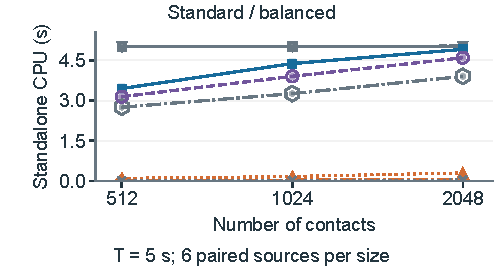
\includegraphics[width=\linewidth]{figures/performance_cpu_scaling_v06__fresh_standard_balanced__standard_balanced.pdf}
    {\small (a)}
  \end{minipage}\hfill
  \begin{minipage}[t]{0.495\textwidth}
    \centering
    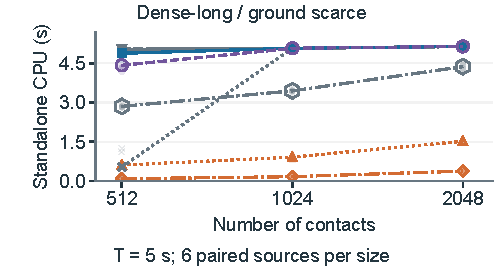
\includegraphics[width=\linewidth]{figures/performance_cpu_scaling_v06__fresh_dense_long_ground_scarce__dense_long_ground_scarce.pdf}
    {\small (b)}
  \end{minipage}
  \par\vspace{1pt}
  
\includegraphics[width=\textwidth]{figures/performance_cpu_scaling_legend_v06.pdf}
  \caption{Measured deployment CPU versus contact count at fixed nominal
  $T=5$ seconds: standard balanced (a) and dense-long ground scarce (b).
  Faint points show six paired sources per size; lines show their mean,
  after within-context seed/member averaging. Warm policies each charge
  the full common CHILS initializer and their own repair; shared graph
  loading remains separate. These are scale comparisons, not anytime traces
  or evidence of LLM speed superiority. Complete gain/coverage matrices
  remain in the supporting report.}
  \Description{Two panels compare actual standalone CPU seconds at contact
  counts 512, 1024, and 2048 for five native method families and warm
  joint witness, EoH-DSL, and Degree policies. Each faint point is one
  paired-source cost; each line joins the six-source means at the three
  sizes. All policies use their frozen identities and native methods
  retain their prescribed seeds. A shared legend identifies eight curves.
  The comparison uses fixed nominal five-second targets and retains
  the full charged common initializer for warm policies.}
  \label{fig:v06_performance_budget}
\end{figure*}
}{}

\subsection{From Full-Residual Evidence to Restricted Patches}
\label{sec:v06-patch-bridge}
A TRAIN bridge examines first patches of 120 common-Degree traces;
106 contain only two vertices. Degree fits all 15 local strict labels;
W joint fits 58/60 output--label positions. Of seven full-strict pairs,
one reverses and three tie under the outside-fixed patch boundary.
Thus full-residual fit cannot certify patch preference or search efficiency.
Complete rows, comparator fits and shortfalls remain in the report.

\subsection{Published-Solver Comparison and Joint-Shift Stress}
\label{sec:v06_performance}

We evaluate all 23 frozen policy identities on 302 contexts at nominal wall
 targets $T\in\{0.1,1,5\}$ seconds. Newly drawn scheduling problems provide
216 endpoints from 108 resource-intervention pairs. Public inputs comprise
25 WDP, three Segmentation, and ten Grids sources from the weighted-clique
benchmark~\cite{mccreesh2017evaluation}, retaining exact weights and complement
orientation. Public source clusters follow fixed withholding within previously
exposed corpora. Two 24-context C3 tracks remain separate exploratory analyses.

Table~\ref{tab:v06-published} displays four predeclared families at $T=5$
against CHILS and ILS~\cite{grossmann2025chils}, M2WIS~\cite{grossmann2024mmwis},
Struction~\cite{gellner2021struction}, and WeightedBR~\cite{lamm2019weighted}.
The deployment comparison keeps the same strong CHILS incumbent and repair
limits for joint witness, Degree, and EoH-DSL policies. Four frozen EoH-DSL
outputs retain their common seed AST~\cite{liu2024eoh}. Every warm policy is
charged the full shared initializer and its own repair cost; nominal targets
are not equal end-to-end deadlines across C++ and compiled Python.

Fresh contact pairs change ground gap $0.5\!\to\!6$ with unchanged
opportunities. They also increase size to 512/1,024/2,048 contacts and vary
weights, durations and density. This combined shift tests deployment stress;
it cannot isolate the effect of unseen gaps. Arbitrary public graphs test
solver compatibility, not satellite constraint adaptation.

Figure~\ref{fig:v06_performance_budget} plots measured CPU against size at
fixed $T=5$ for two predeclared contact families. Points retain paired-source
costs; lines join their means. Complete cold/warm reward, coverage and all
13-family/three-target matrices remain in the supporting report. Cohort
reward means require every member to return a successful feasible schedule;
partial means cannot establish superiority over fully covered comparators.
No test outcome changes a program, budget or displayed family.

The common optimization backbone retains its feasible incumbent while the
synthesized policies provide refined decision representations. The deployment
results illustrate this separation between information adequacy and achieved
schedule quality; they do not establish an incremental LLM quality gain.


\section{Discussion}
\label{sec:discussion}
Representation adequacy, scalar fitting and search effectiveness are distinct.
Repairing a quotient enlarges what a rule can express. All TRAIN patch searches
finish exactly: priorities change search order but final rewards coincide.
This lack of TRAIN quality gain precedes distribution shift, so mismatch alone
cannot explain it. Information repair has not demonstrated optimizer benefit.

Witness conditioning improves gate yield; relations-only programs retain
stronger scalar fit and W costs are not lower. Warm deployment establishes no
incremental reward gain over Degree or EoH. Only ground-gap changes are paired;
small unit-weight TRAIN/TEST share resource regimes. Large tests jointly change
scale, weight and density. They establish neither isolated configuration gain
nor recurring large-scale decision semantics. Boundary-aligned evidence and
matched large-scale training require further study. Renaming contradictions,
Grids cohort failures, cold losses and detailed costs remain in the report.

Finite DAG representability ensures neither bounded-grammar fit nor transfer.
Guarantees also apply to enumerated proposals; LLMs construct, not certify.
Heterogeneous weights change observed distinctions~\cite{mccreesh2017evaluation}.
Additive optimality and nominal targets differ from minimum runtime and equal
computation. Corpus exposure, unmatched compute and identifier ties further
delimit generalization claims.

\section{Conclusion}
\label{sec:conclusion}
Certified representation--rule refinement diagnoses missing information before
rule repair. Sound completion bounds and quotient witnesses direct typed
LLM proposals, complemented by a scoped additive-cost guarantee. Witness
feedback improves observed gate yield; joint selection raises withheld fit
within W. Frozen classical deployment separates these information benefits
from optimizer quality, enabling targeted constraint adaptation.

\clearpage
\balance
\bibliographystyle{ACM-Reference-Format}
\begingroup
\interlinepenalty=10000
\bibliography{references_v03,references_extension_v05,drafts/v06/new_references}
\endgroup
\end{document}
